\documentclass[11pt]{article}
\usepackage[left=1in, right=1in, top=1in, bottom=1in]{geometry}
\usepackage{fancyhdr}
\usepackage{hyperref}
\usepackage{graphicx}
\usepackage{float}

\pagestyle{fancy}
\lhead{Chen, Zimmerman}
% zero-index page numbers
\setcounter{page}{0}
\rhead{\thepage}

\begin{document}
\thispagestyle{empty}
\noindent
\begin{minipage}[width=0.7\linewidth]{0.7\linewidth}
  Howard Chen, Jacob Zimmerman\\
  hhchen@andrew.cmu.edu, jezimmer@andrew.cmu.edu\\
  10/30/2014
\end{minipage}
\hfill
\begin{minipage}[width=0.3\linewidth]{0.3\linewidth}
  \flushright
  15-221\\
  Fall 2014\\
  Section B
\end{minipage}

\begin{center}
  Written Homework 4\\
  How to Use ExplainShell for Chrome\\
  (Note: Mr. Keating gave us a two-day extension)
\end{center}
\newpage

\tableofcontents

\newpage

\section{Introduction}

\subsection{Motivation}
Many times, when using the terminal, you encounter lines of shell code that make no sense. Fortunately, the site \href{http://explainshell.com/}{ExplainShell.com} helps by looking up particular commands and flags and explaining them. However, having to copy, switch tabs, and then paste can distract from what you were doing in the first place. The Chrome extension ExplainShell for Chrome alleviates this issue. In this tutorial, we'll describe the process of installing and using ExplainShell for Chrome.


\subsection{Overview}
Following this tutorial will take \textbf{no longer than 10 minutes}. All in all, it's a \textbf{total of 6 steps}. You're a perfect candidate for this tutorial if you often work in a terminal or command line environment. All you need is a computer with the Google Chrome web browser installed! Let's get started.

\newpage

\section{Installation}
First we need to install ExplainShell for Chrome. We can do this through the Chrome Webstore.

\subsection{Navigate to the Chrome Webstore}
Within Chrome, navigate to the URL \url{https://chrome.google.com/webstore/}. This is illustrated in Figure~\ref{chrome-webstore}.

\vspace{0.2in}
\begin{figure}[H]
  \begin{center}
    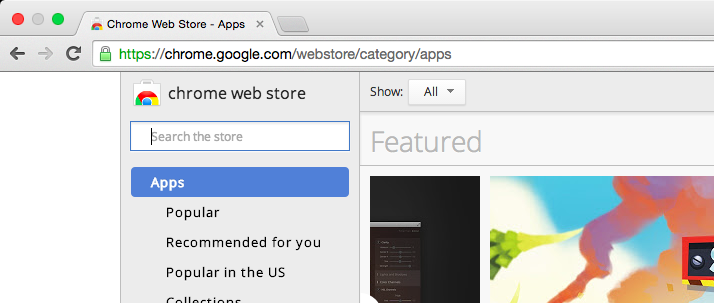
\includegraphics[width=\textwidth,height=\textheight,keepaspectratio]{01chrome-webstore}
  \end{center}
  \caption{Navigating to the Chrome Webstore}
  \label{chrome-webstore}
\end{figure}
\vspace{0.2in}

\subsection{Search for ExplainShell for Chrome}
In the search box on that page, \textbf{search for ``ExplainShell for Chrome''}. If you're having trouble locating the search box, be sure to check out Figure~\ref{search-box}.

\vspace{0.2in}
\begin{figure}[H]
  \begin{center}
    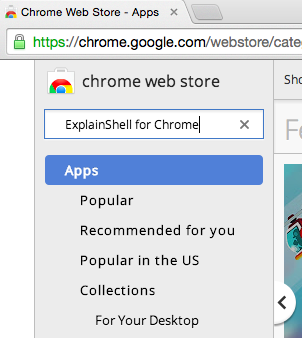
\includegraphics[width=2in, keepaspectratio]{02search-box}
  \end{center}
  \caption{Search for ``ExplainShell for Chrome''}
  \label{search-box}
\end{figure}
\vspace{0.2in}

\subsection{Install the Extension}
Your search should have turned up the correct extension. At the time of writing this tutorial, this query returns only one result. Be sure to check Figure~\ref{install} if your search returned multiple results in order to disambiguate between the results.

\mbox{}\\
\noindent
Click on the \textbf{blue ``+ Free'' button} to the right to download and install the extension.

\vspace{0.2in}
\begin{figure}[H]
  \begin{center}
    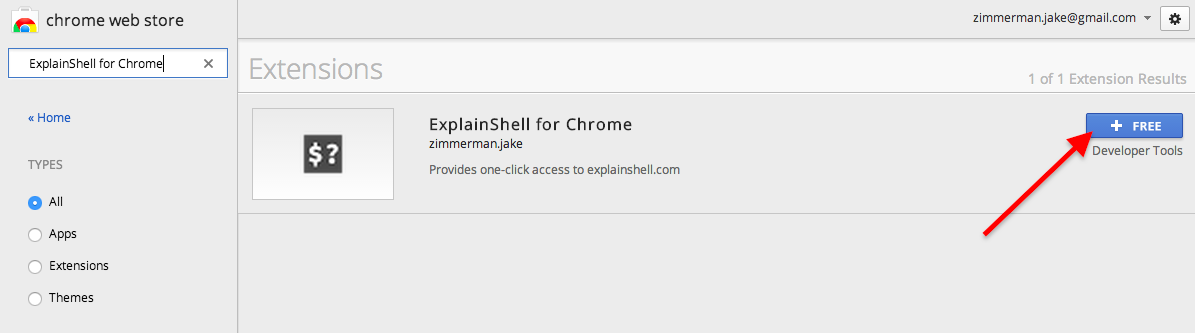
\includegraphics[width=\textwidth, height=\textheight, keepaspectratio]{03install}
  \end{center}
  \caption{Click the button pointed to by the red arrow to install.}
  \label{install}
\end{figure}
\vspace{0.2in}

\subsection{Confirm the Installation}
After clicking the button, Chrome will ask you if you really mean to install the extension. \textbf{Click ``Add'' to continue} and it should install in seconds.

\vspace{0.2in}
\begin{figure}[H]
  \begin{center}
    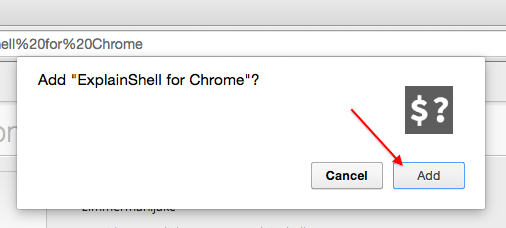
\includegraphics[height=2in, keepaspectratio]{04confirm}
  \end{center}
  \caption{Click the button pointed to by the red arrow to confirm.}
  \label{confirm}
\end{figure}
\vspace{0.2in}

\section{Usage}
The following steps will describe how to actually use ExplainShell for Chrome to look up a line of shell code.

\subsection{Context}
Let's say that I'm interested in installing the Homebrew package manager. I've navigated to their site and I see that to install it, they want me to run a particular line of code. Curious as to what this line does, I decide to use ExplainShell for Chrome to look it up.

\mbox{} \\
\noindent
This is just one example of how to use ExplainShell for Chrome. If you happen to have a different site where you know there's a line of shell code, feel free to follow along there! For reference though, you can see what my screen looks like in Figure~\ref{brew}.

\vspace{0.2in}
\begin{figure}[H]
  \begin{center}
    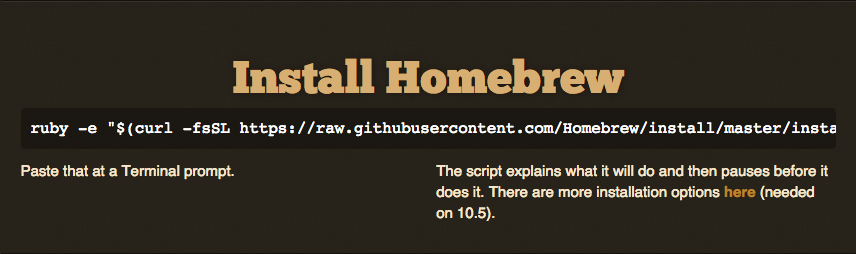
\includegraphics[width=\textwidth, height=\textheight, keepaspectratio]{05brew}
  \end{center}
  \caption{I'll be using the site \url{http://brew.sh} to demonstrate.}
  \label{brew}
\end{figure}
\vspace{0.2in}

\subsection{Select the text and look it up}
Using the extension is incredibly simple. 

\begin{enumerate}
  \item Select the text
  \item Right click what you just highlighted (the text should remain highlighted)
  \item Locate and click on the menu item that reads ``Lookup on explainshell.com''. This will take you to explainshell.com in a new tab.
\end{enumerate}

All of these steps can be seen in Figure~\ref{lookup}. \textbf{If you don't see the item} in the menu that pops up, it's possible that the Chrome extension failed to install. You can verify that the extension is there by navigating to \url{chrome://extensions} and checking if you see an extension named ``ExplainShell for Chrome''. If not, repeat the installation steps.

\vspace{0.2in}
\begin{figure}[H]
  \begin{center}
    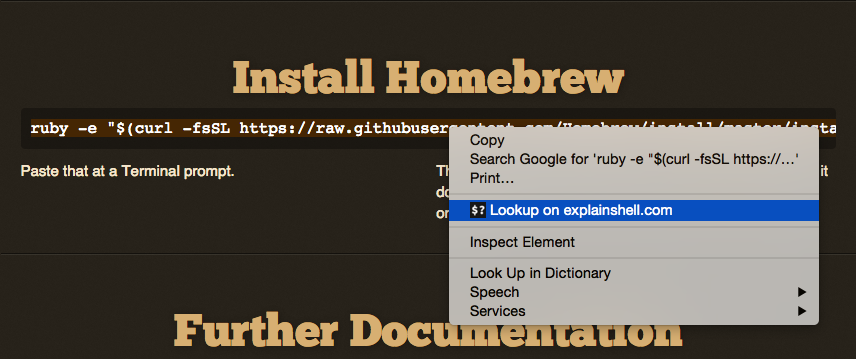
\includegraphics[width=\textwidth, height=\textheight, keepaspectratio]{06lookup}
  \end{center}
  \caption{Click the menu item highlighted above to jump to explainshell.com}
  \label{lookup}
\end{figure}
\vspace{0.2in}

\subsection{ExplainShell.com}

After clicking, you should see ExplainShell.com open in a new tab. Peruse the documentation, and close the window when done. Simple!

\vspace{0.2in}
\begin{figure}[H]
  \begin{center}
    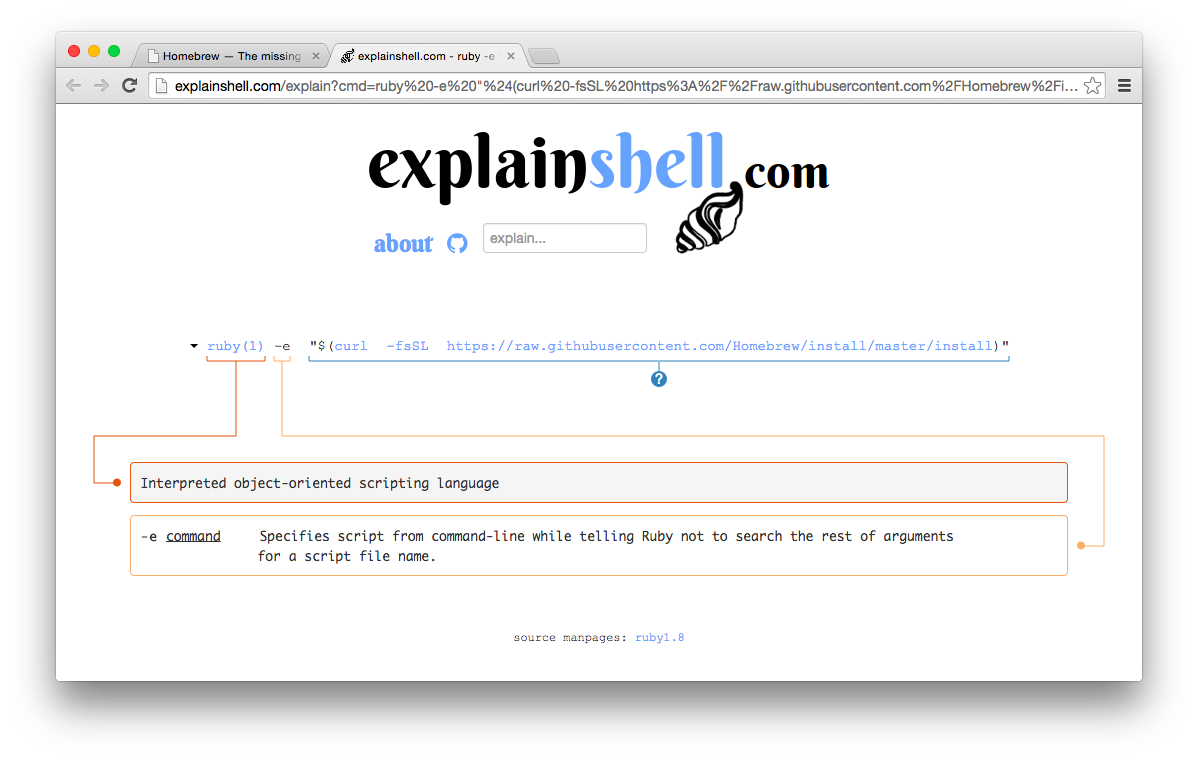
\includegraphics[width=\textwidth, height=\textheight, keepaspectratio]{07explainshell-website}
  \end{center}
  \caption{You should see ExplainShell.com after the new tab opens.}
  \label{explainshell-website}
\end{figure}
\vspace{0.2in}

\section{Summary}
At this point, you should have all the tools you need to install and use the ExplainShell for Chrome extension. If, however, you do experience an issue while working with the extension, be sure to report it here: \url{https://github.com/justingallagher/explainshell-for-chrome/issues}. We'll guide you through the process of resolving your issue and implement any fixes as necessary. Thanks!

\end{document}
